
\begin{figure}[!ht]
\begin{subfigure}{1\textwidth}
  \centering
  % include second image
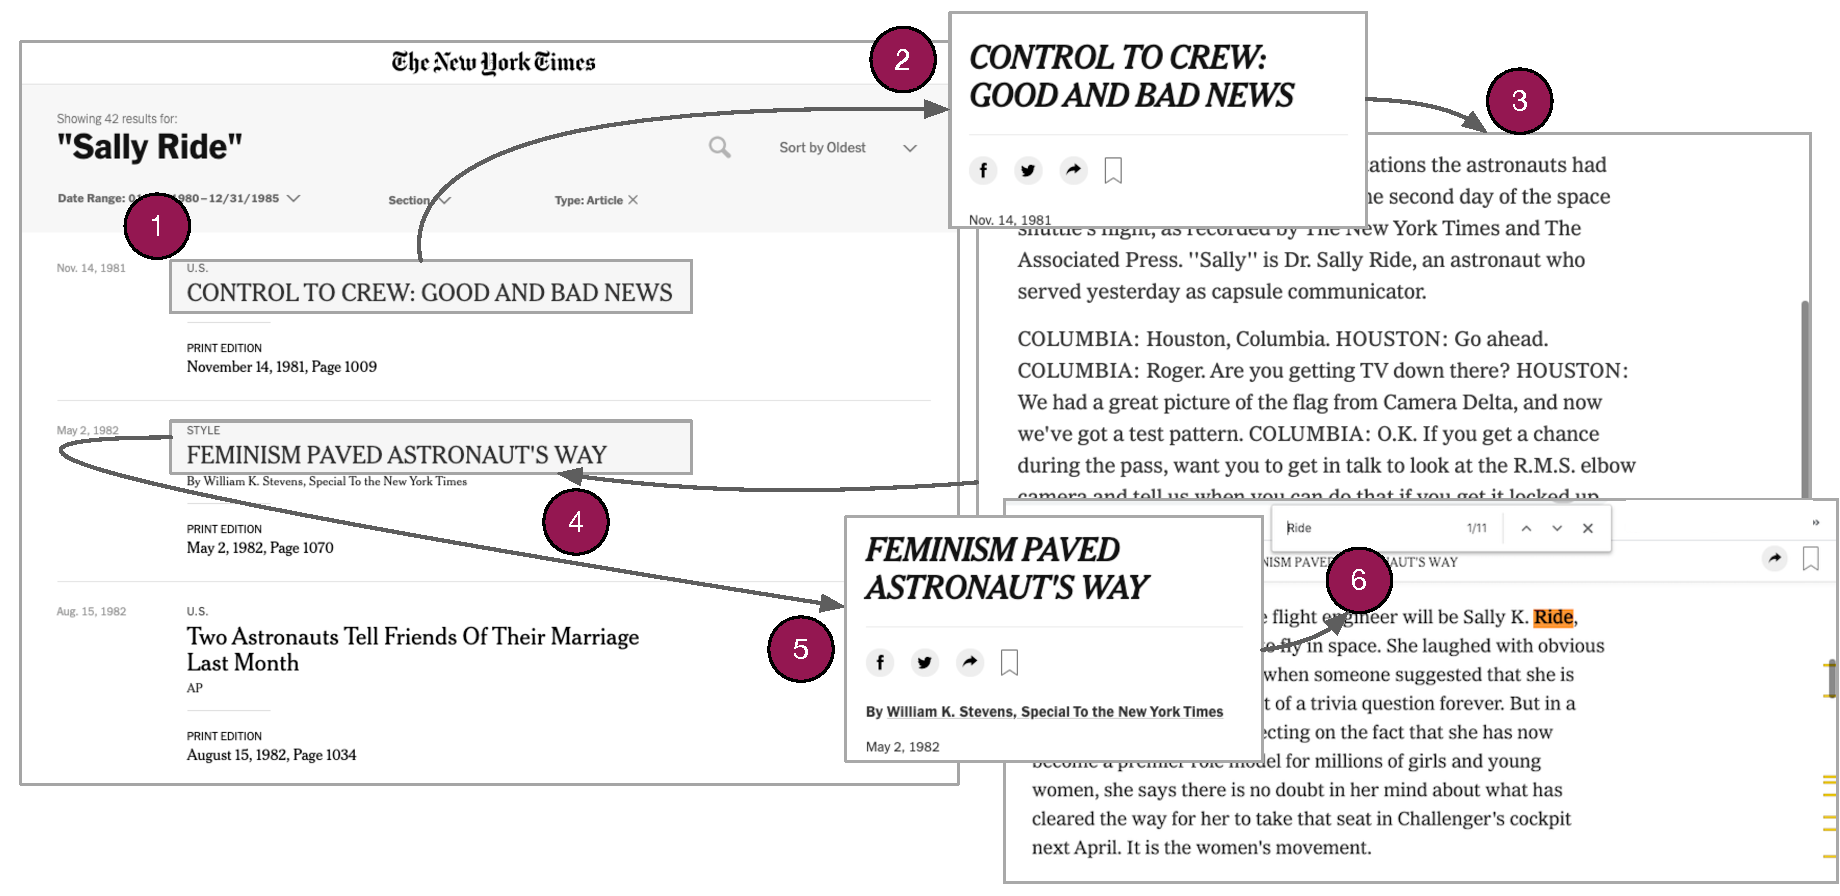
\includegraphics[width=.71\linewidth]{figures/workflow_fig/open_locate_loop_nyt.pdf}
  \subcaption{
% \footnotesize %  uncomment for thesis
  A user investigates Sally Ride by performing {\burdensome~and analysis} using the \textit{New York Times} web archive \cite{nytwebsite}, a baseline keyword document search interface (Section \ref{s:baseline}). They first (1) click the top headline on the search engine results page (left) in order to (2) {open} a document in a new tab (shown on the right) and then (3) scroll down to {locate} mentions of ``Ride'' in the linked news story. The user {reads} and analyzes these mentions and then (4) context switches to the second document by clicking the second headline on the results page. This (5) opens a new story in a new tab. For this second document, they (6) use a search in document feature \cite{chromeF} (i.e.\ \texttt{Control+F}) to help {locate} mentions of ``Ride'' within the story.
}\label{f:field_study_1} \vspace{.25cm}
\end{subfigure}
\begin{subfigure}{1\textwidth}
  \centering
  % include first image
  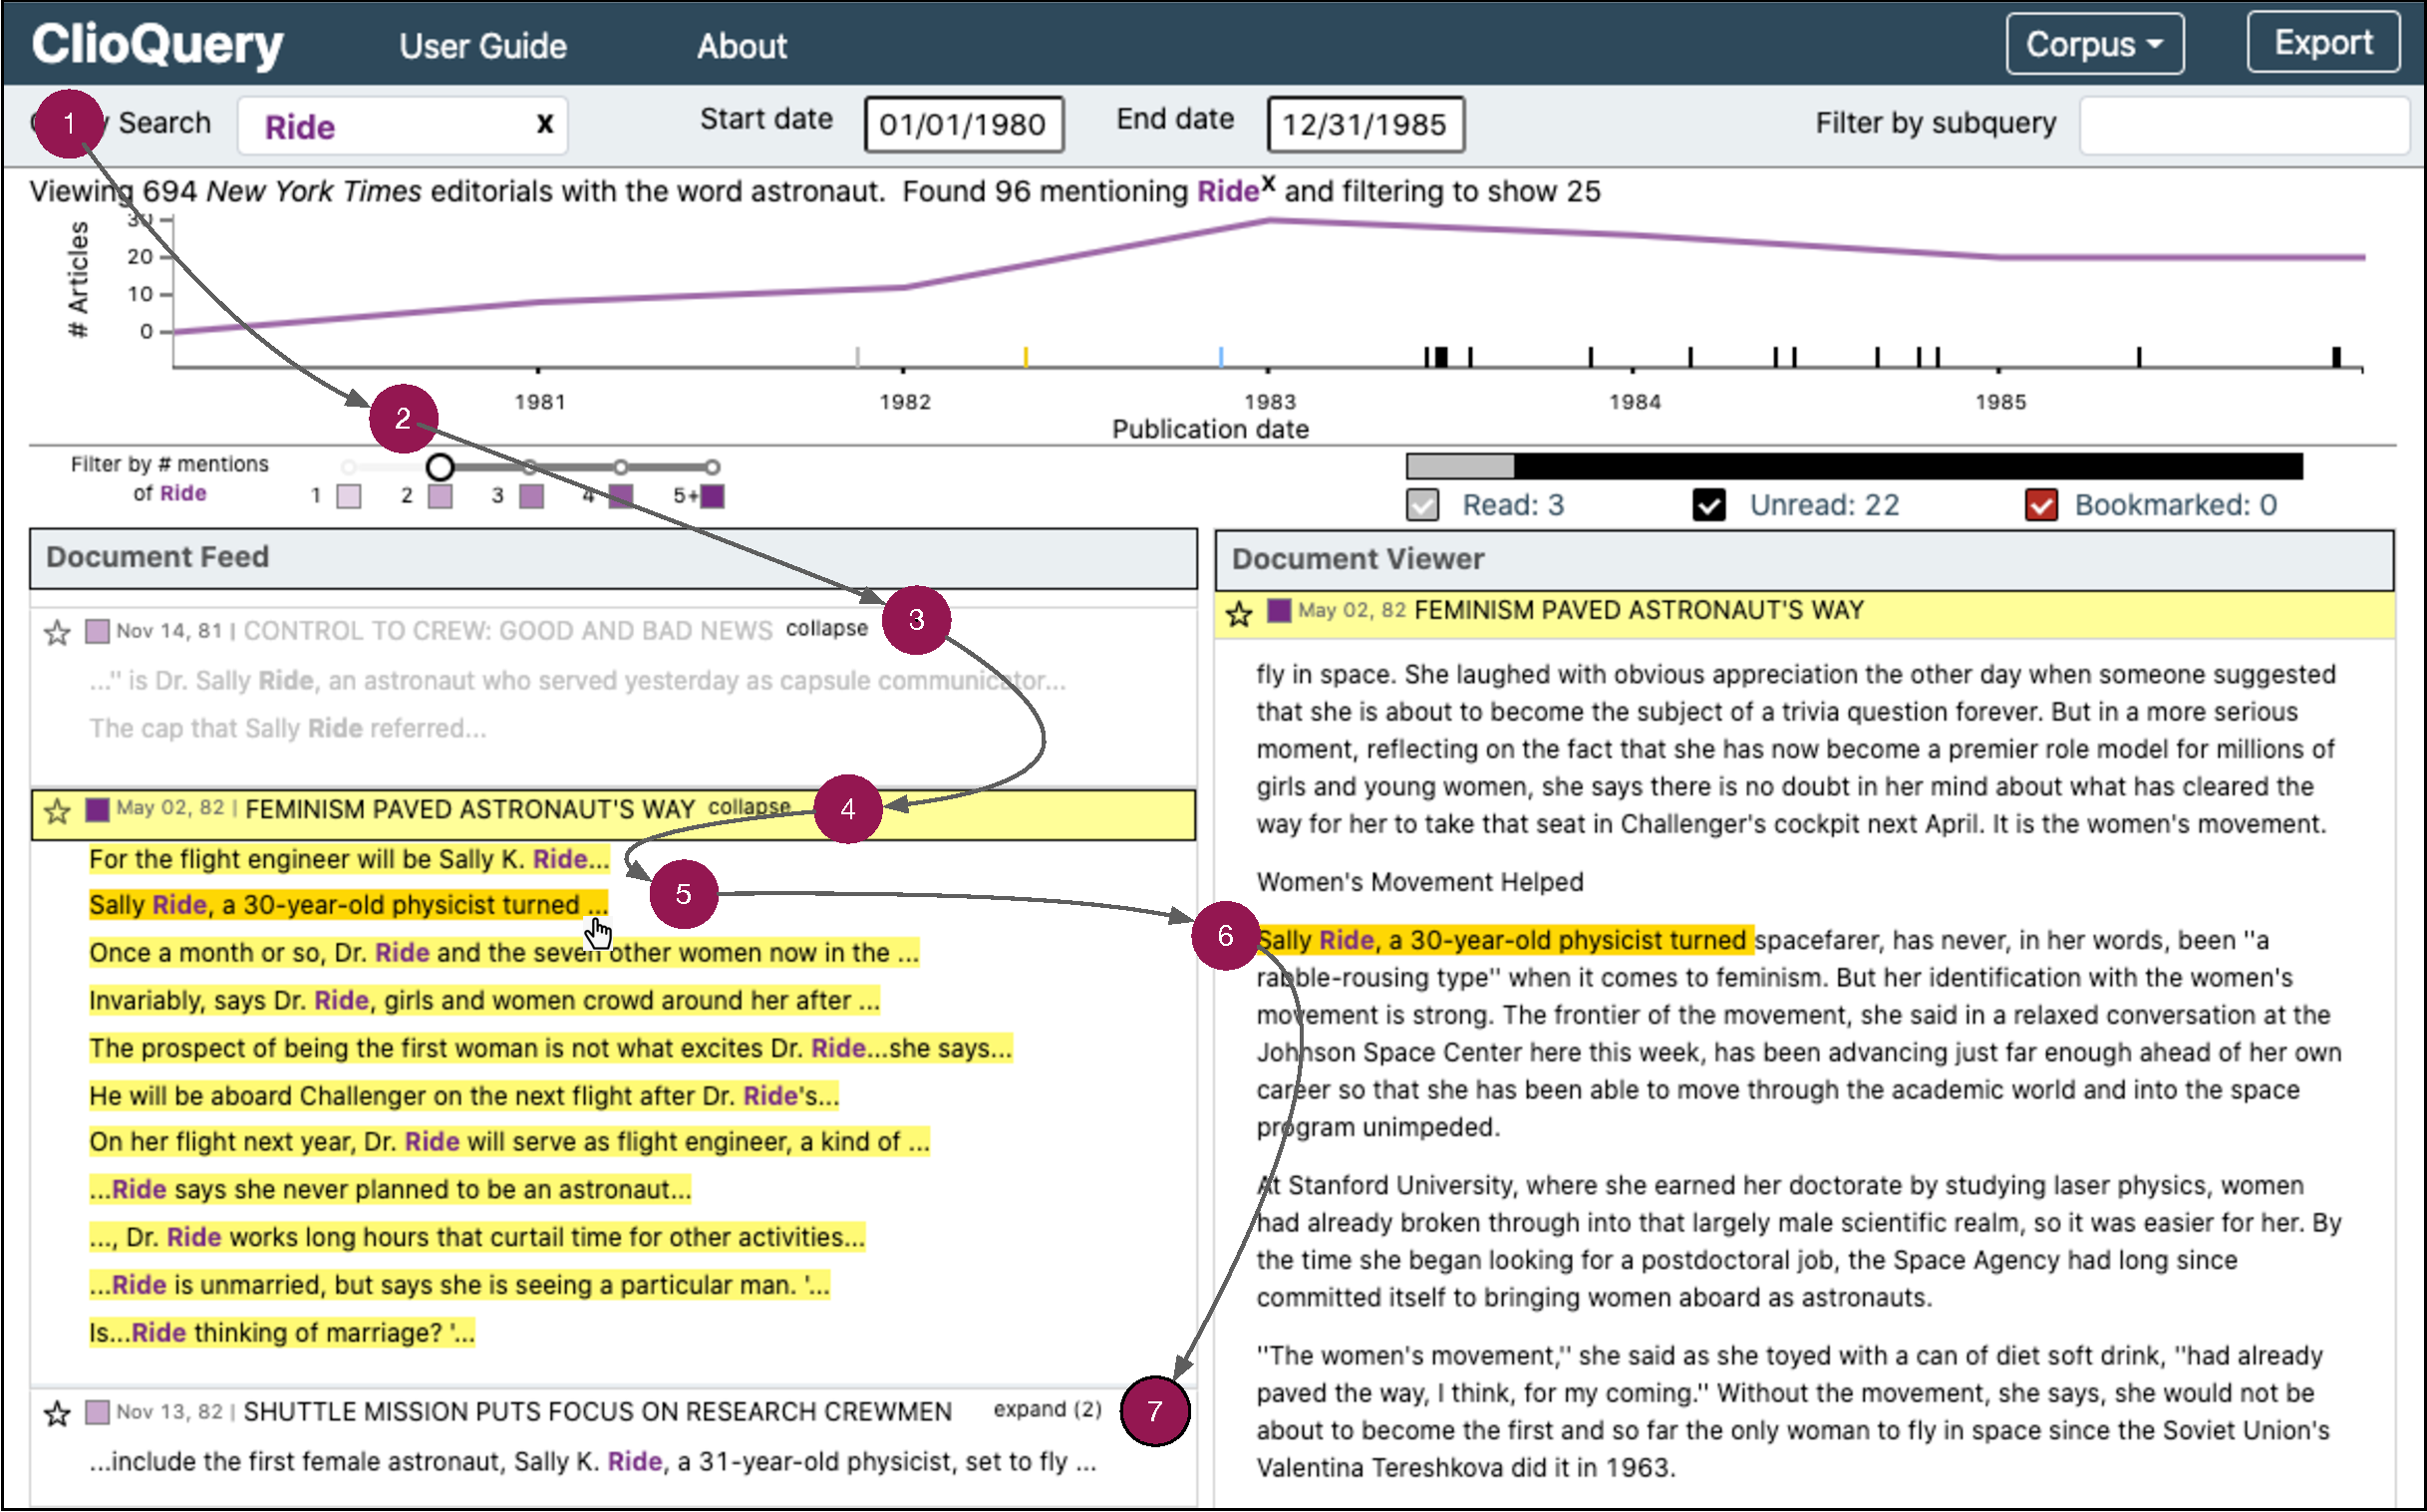
\includegraphics[width=.683\linewidth]{figures/workflow_fig/open_locate_loop_CC.pdf}  
 \subcaption{
% \footnotesize %  uncomment for thesis
 A user (1) searches for ``Ride'' using \ours~and (2) sets the filter-by-count slider to limit results to stories with at least two mentions of ``Ride''. The user then clicks the expand/collapse button on two news stories (3 and 4) to review all mentions of Ride from each story in the Document Feed. They then (5) click one shortened sentence mentioning ``Ride'' (6) to read it within the context of the full original document in the linked Document Viewer, with help from automatic in-text highlighting. The user then prepares to (7) click expand to review additional mentions of Ride in the next story.}\label{f:field_study_2}
\end{subfigure}
%In this figure, history tracking is disabled; articles the user has already read would normally be shown in grey.
\caption[A workflow with \ours~and a \Baselongname~tool]{
% \footnotesize % uncomment for thesis
Reviewing mentions of U.S.\ astronaut Sally Ride in~\textit{The New York Times}, using \ours~(bottom) and a \Baselongname~tool (top). 
This particular example comes from our field study (Section \ref{s:fieldstudy}), where one historian commented on the advantages of the \ours~interface over a baseline \Baselongname~system.
\textit{ ``What can I do here [with \ours] that I can't do there [with \textit{New York Times} search]?"} she said. 
\textit{``It's exploring this left-hand Document Feed.''}
Where \ours~facilitates quick and comprehensive review of all query mentions, the \Baselongname~tool requires the user to read unnecessary passages and context switch across documents.
}\label{f:field_study_loop}
\end{figure}
